\documentclass{article}
\usepackage[margin=1in]{geometry}
\usepackage{graphicx}
\usepackage{amsmath}
\usepackage{amssymb}
\usepackage{mathtools}
\usepackage{cite}

\def\ins{\hbox{$\circ$}\kern-1.5pt\hbox{$\to$}\kern -1pt\hbox{$\circ$}}
\def\sec{\hbox{$\bullet$}\kern-1.5pt\hbox{$\to$}\kern -1pt\hbox{$\bullet$}}
\def\auth{\hbox{$\bullet$}\kern-1.5pt\hbox{$\to$}\kern -1pt\hbox{$\circ$}}
\def\conf{\hbox{$\circ$}\kern-1.5pt\hbox{$\to$}\kern -1pt\hbox{$\bullet$}}

\newcommand{\mono}[1]{\textrm{\tt #1}}

%---------
\usepackage{epigraph}
\usepackage{tabularx}
\usepackage{booktabs}
\usepackage{multirow}
\usepackage[table,xcdraw]{xcolor}
\usepackage{adjustbox}
\usepackage{tablefootnote}

\definecolor{color1}{RGB}{0,0,90} % Color of the article title and sections
\definecolor{color2}{RGB}{0,20,20} % Color of the boxes behind the abstract and headings
\definecolor{keys1}{rgb}{0.0, 0.29, 0.33}
\definecolor{keys2}{rgb}{0.25, 0.7, 0.55}
\definecolor{keys3}{rgb}{0.1, 0.3, 0.4}
\definecolor{keys4}{rgb}{0.21, 0.46, 0.53}
\definecolor{strings}{rgb}{0.0, 0.47, 0.44}
\definecolor{comments}{rgb}{0.4, 0.4, 0.5}
\definecolor{terminaltext}{rgb}{1,1,1}
\definecolor{terminalbackground}{rgb}{0.2,0.2,0.25}

%----------------------------------------------------------------------------------------
%	BLOCKS
%----------------------------------------------------------------------------------------

\usepackage[framemethod=TikZ]{mdframed}
\newcounter{definition}[section]\setcounter{definition}{0}
\newcommand{\thedef}{\arabic{section}.\arabic{definition}}
\newenvironment{definition}[2][]{%
    \refstepcounter{definition}
 
    % Code for box design goes here.
	\ifstrempty{#1}%
	% if condition (without title)
	{\mdfsetup{%
	    frametitle={%
	        \tikz[baseline=(current bounding box.east),outer sep=0pt]
	        \node[anchor=east,rectangle,fill=color2!10]
	        {\strut Definition~\thedef};}
	    }%
	% else condition (with title)
	}{\mdfsetup{%
	    frametitle={%
	        \tikz[baseline=(current bounding box.east),outer sep=0pt]
	        \node[anchor=east,rectangle,fill=color2!10]
	        {\strut Definition~\thedef:~#1};}%
	    }%
	}%
	% Both conditions
	\mdfsetup{%
	    innertopmargin=10pt,linecolor=color2!10,%
	    linewidth=1pt,topline=true,%
	    frametitleaboveskip=\dimexpr-\ht\strutbox\relax%
	}
 
\begin{mdframed}[]\relax}{%
\end{mdframed}}

%----------------------------------------------------------------------------------------
%	HYPERLINKS
%----------------------------------------------------------------------------------------

\usepackage{hyperref} % Required for hyperlinks

\hypersetup{
	hidelinks,
	colorlinks,
	breaklinks=true,
	urlcolor=color2,
	citecolor=color1,
	linkcolor=color1,
	bookmarksopen=false,
	pdftitle={Title},
	pdfauthor={Author},
}
%---------



\title{Formalizing Social Engineering attacks in the Symbolic Model}

\begin{document}
\maketitle
\tableofcontents

%------------------------------------------------

\section*{Introduction} % The \section*{} command stops section numbering

\addcontentsline{toc}{section}{Introduction} % Adds this section to the table of contents

\epigraph{Security protocols are three-line programs that people still manage to get wrong}{Roger M. Needham}

Today's digital infrastructure is increasingly reliant on cryptographic protocols in order to function correctly and efficiently while mitigating the risks of intrusion by malicious parties. Online applications are overtaking traditional physical offices in the name of efficiency; but while mimicking the often decades-old tasks themselves (like purchasing public transportation tickets or voting) in the cyberspace is generally not a big deal on itself, guaranteeing the security of these virtual processes against emerging digital threats demands a lot more research effort. Formal verification tools allow us to construct checkable models of cryptographic protocols and to verify them against well-defined threat models to ensure that such exchanges do not hide any flaws in their design, however, they often rely on strong assumptions regarding the caution and knowledge of the involved users. In this paper, we want to introduce a possible solution for a more complete analysis of protocols which heavily rely on partecipants' input based on the ideas of human knowledge and human error.

The essay is structured as follows: in section \ref{sec:SymbolicModel} we will briefly introduce one of such formal verification models, in section \ref{sec:TamarinOverview} we will give an introduction to the Tamarin prover (mainly from a user's perspective), while in the following section \ref{sec:SocialEngineering} we will show how we can formalize Social Engineering attacks using said tool's syntax in a very intuitive way. Finally, in section \ref{sec:Conclusions} we will summarize the contents of this paper.

\section{The Dolev Yao model}\label{sec:SymbolicModel}

When dealing with the verification of internet protocols, two (main) paradigms are used to formally prove the security properties of both new and already established message exchanges: the \textit{computational} and the \textit{symbolic model}. The first, initially introduced by Goldwasser, Micali \cite{goldwasser}, Rivest \cite{rivest}, Yao \cite{yao} and others, treats messages as bitstrings, cryptographic primitives as endomorphisms mapping objects in the space of bitstrings and the adversary as a probabilistic Turing machine. Within this model, given a security parameter (such as an encryption key) and a property (formula) that needs to be verified, the adversary must find a polynomial-time algorithm with respect to the size of the parameter that makes the formula false. If the probability of such procedure to work is negligible, then the property is considered as proved. This model manages to resemble real-world cryptography pretty closely, but specifing and verifying its theories can easily become a tedious and lengthy process.

At the cost of accuracy, the symbolic model (also known as the Dolev-Yao model \cite{DolevYao}) abstracts from real-world cryptography operations by substituting actual crypto primitives with term-algebras. Encryption schemes are easily formalized through binary isomorphisms: for example, given a secret key $k$ and the relevant pair of cryptographic encryption and decryption function symbols $\textrm{senc}_k$, $\textrm{sdec}_k$ and $1$, symmetrical cryptography is defined through the following identity:
\begin{equation}\label{eq:SymmetricEncryptionIdentity}
    \textrm{sdec}_k\ \textrm{senc}_k = 1
\end{equation}

Only the entities that are in possess of $k$ are able to encrypt or decrypt any message (term) with it \cite{BBSecurityProtocolVerification}: this hypothesis is known as \textit{perfect cryptography}.

Similarly to equation \ref{eq:SymmetricEncryptionIdentity}, asymmetric encryption is modeled through the following identity:
\begin{equation}\label{eq:AsymmetricEncryptionIdentity}
    \textrm{adec}_{pr}\ \textrm{aenc}_{pub} = \textrm{adec}_{pub}\ \textrm{aenc}_{pr} = 1
\end{equation}

In this case, we do not consider a single key used for both encryption and decryption $k$, but instead an entangled pair of keys $pr$ and $pub$.

Given a message $M$ and its image $\textrm{senc}_k\ M$ (or, $\textrm{aenc}_{pub}\ M$), we assume that it is impossible for an attacker who does not know $k$ (or $pr$) to:

\begin{itemize}
    \item guess or bruteforce $k$ (or $pr$);
    \item manipulate $\textrm{senc}_k\ M$ (or $\textrm{aenc}_{pub}\ M$)
    \item infer any information about $M$ from $\textrm{senc}_k\ M$ \\(or $\textrm{aenc}_{pub}\ M$).
\end{itemize}

This set of hypotheses represents both the strength and weakness of this paradigm: from a modeling point of view, the abstractions introduced effectlively strip down protocols of their low-level implementation complexity, keeping only the required cryptographic primitives, and thus allowing for far easier formalization and verification processes. Long and complex message exchanges between multiple parties are manageable within this model and, as we will soon show, various provers have been proposed with this purpose during recent years. On the other hand, by simplyfing cryptography down to only algebraic terms, this model does not take into consideration neither possible bad implementation choices nor real-world attacks regarding the cryptographic primitives actually used. The computational model, by being less abstract, clearly covers a wider spectrum of risk scenarios, but with an non-negligible added complexity and still without being considered a completely inclusive paradigm (we can trivially think about side channel attacks, which are not being included in any threat model by definition).

Coming back to the Dolev-Yao model, a protocol is formalized as a series of algebraic terms (messages) exchanged by abstract machines (clients) through an attacker-controlled network. We assume that any connection can be eavesdropped by a malevolent agent that is also able to intercept, modify, forge and drop messages on the fly (but always following the perfect cryptography constraints described). After formalizing a protocol, its security goals can be expressed as:

\begin{itemize}
    \item \textit{Trace properties}: invariants that should hold for each possible execution of the protocol;
    \item \textit{Observational equivalence properties}: properties that an attacker should not be able to distinguish between two different runs of the protocol.
\end{itemize}

\subsection{Computational limits of the symbolic model}

In order to streamline the proof of security properties belonging to a certain protocol in the symbolic model, multiple automatic tools were proposed \cite{SoK}. In order to verify security goals, these softwares have to compute the set of terms that an attacker is able to deduce from the network while (possibly) multiple runs the protocol are executing; since such set can possibly be unbounded, the general task can quickly become undecidable and suffer of the infinite state space problem: we can have an infinite number of sessions for each protocol, each one with an unbounded amount of nonces and messages of unlimited size. Without bounding at least two of these sources of infinity, termination can not be guaranteed by any tool in this category \cite{undecidability}.

\begin{figure*}[t]
    \centering
    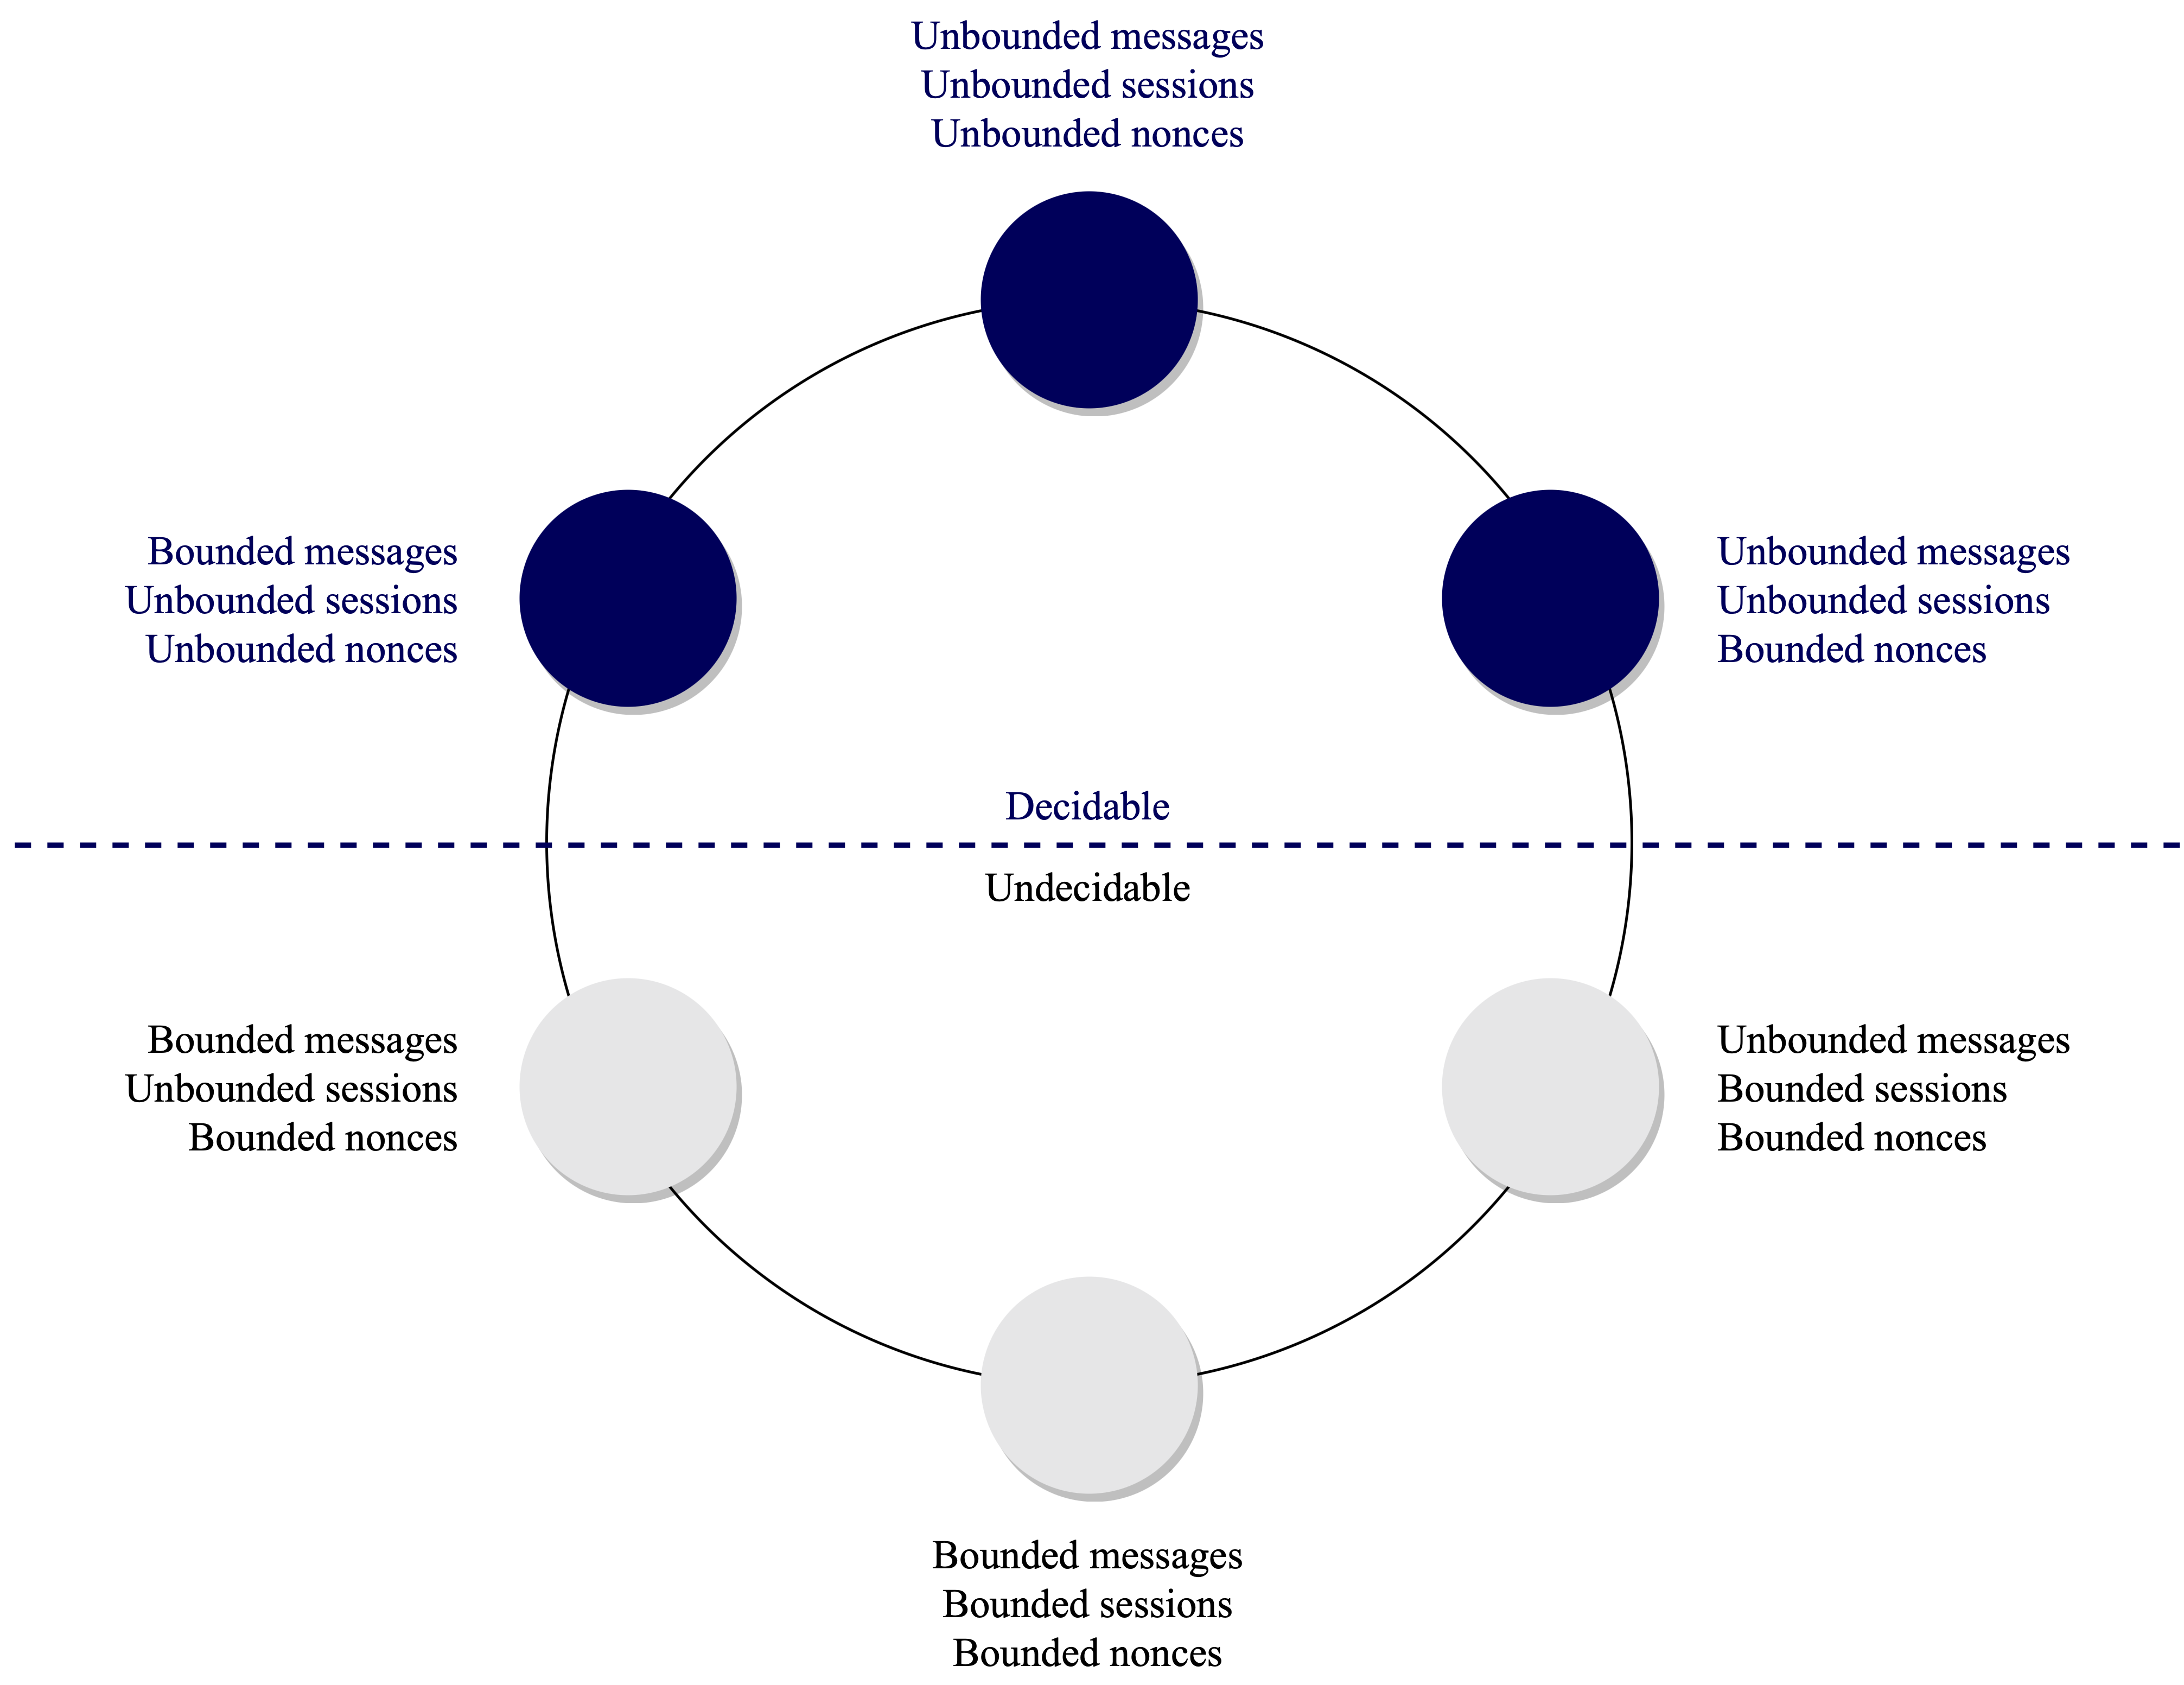
\includegraphics[width=0.8\textwidth]{images/undecidability.png}
    \caption{Decidability in symbolic verification. Image inspired by N. Vitacolonna's presentation \cite{PresentazioneVitacolonna}}
\end{figure*}


In particular, as shown by N. Durgin et al. \cite{ComplexityOfBoundedSecurity}, by restricting different sources we can ensure to reduce the model checking problem to different complexity classes:

\begin{itemize}
    \item if we limit the number of nonces and messages, we end up with a DEXP-complete problem;
    \item if we restrict the number of sessions and nonces, the problem will still be affected from unbounded state space, but its solution will be NP-complete; this workaround was adopted by a variety of tools such as Cl-AtSe \cite{clAtse}, OFMC \cite{ofmc} and SATMC \cite{satmc}.
\end{itemize}

Alternatively to bounding the sources of infinity, some software address undecidability by requiring human input (for example, Tamarin Prover \cite{tamarinIntroduction} features an interactive mode that allows the user to decide which security goals prioritize based on intermediate constraint systems, as we will see in \ref{subsec:tamarinGui}), returning inconclusive results (for example, ProverIf \cite{proverifIntroduction} may return an invalid attack trace) or even allowing non-termination.

\section{Tamarin Prover Overview}\label{sec:TamarinOverview}

In 2012, researchers at ETH introduced a new symbolic verification software, the Tamarin prover. Such tool provides an automated search for attacks, advanced protocol analysis techniques, and an interactive theorem proving approach that enables security experts to manually guide the proof process. We will now do a quick overview of its syntax, semantics and internal functioning; please refer to S. Meier's \cite{meierThesis} and B. Schmidt's \cite{schmidtThesis} PhD thesis and their introductory paper \cite{TamarinFoundations} for further information about the theoretical foundations regarding this tool, as long as its official manual \cite{tamarinManual} to solve any doubts about its use.

\subsection{Term algebra}

As explained in \ref{sec:SymbolicModel}, the Dolev-Yao model formalizes cryptographic messages within a term algebra; thus, in order to introduce Tamarin's syntax, we firsly have to take a look at (some) of the theoretical foundations behind is formalism. 

\begin{definition}[Signature]
    A A signature $\Sigma$ is a finite set of functions of defined arity.
\end{definition}

Signatures are fundamental, since are the building blocks of our theory. As we will soon see, all the algebraic terms we introduced before (for example in equations \ref{eq:SymmetricEncryptionIdentity} and \ref{eq:AsymmetricEncryptionIdentity}) will be expressed as function symbols.

\begin{definition}[$\Sigma$-terms]
    G Given a signature $\Sigma$ and a set of variables $\chi$, with $\Sigma \cap \chi = \varnothing$ we can define the set of $\Sigma$-terms $\mathcal{T}_{\Sigma}(\chi)$ as the minimal set such that

    \begin{itemize}
        \item $\chi \subseteq \mathcal{T}_{\Sigma}(\chi)$
        \item $t_1,...,t_n \in \mathcal{T}_{\Sigma}(\chi) \land f/n \in \Sigma \implies f(t_1,...,t_n) \in \mathcal{T}_{\Sigma}(\chi)$
    \end{itemize}

    Note that $f/n$ indicates a function $f$ of arity $n$.
\end{definition}

While in this introduction we will deal with domain-agnostic logical terms, in practice Tamarin discriminates between 3 different types of terms to model various assumptions on different pieces of knowledge:

\begin{itemize}
    \item \textit{Fresh} (groud) terms are prefixed by a \textasciitilde{} and model information that we can assume a party can check for freshness.
    \item \textit{Public} names are juxtaposed by a \$ and formalize ground information that any party within the network knows.
    \item \textit{Normal} terms are any form of term: fresh, public or built upon function symbols.
\end{itemize}

$\Sigma$-terms allow us to recursively define algebraic terms starting from ground istances of variables. In real life we are able to combine multiple cryptographic primitives in order to build protocol messages: analogously, this set is made up of all the (countably infinite) possible combinations of function applications starting from ground terms.

Clearly, we need now a way to "compare" messages: as we previously explained in equations \ref{eq:SymmetricEncryptionIdentity} and \ref{eq:AsymmetricEncryptionIdentity}, the decryption of the encryption of any message (of course with the correct keys) must match the message itself. Similarly, all the primitives we will introduce must have some mechanism to check whether two terms belonging to a given set $\mathcal{T}_{\Sigma}(\chi)$ match each other or not.

\begin{definition}[Substitution]
    G Given a signature $\Sigma$ and a set of variables $\chi$, with $\Sigma \cap \chi = \varnothing$, a substitution is a function $\sigma: \chi \rightarrow \mathcal{T}_{\Sigma}(\chi)$.
\end{definition}

In our case, we do not only want to be able to build (and compare) terms upon ground instances of variables, but also build them upon other terms. As a consequence, we must generalize the definition of substitution:
    
\begin{definition}[Mapping]
    G Given a function $f/n \in \Sigma$, a mapping $\sigma':\mathcal{T}_{\Sigma}(\chi) \rightarrow \mathcal{T}_{\Sigma}(\chi)$ is an extension of a substitution $\sigma: \chi \rightarrow \mathcal{T}_{\Sigma}(\chi)$ such that
    \begin{equation*}
        f(t_1,...,t_n)\sigma' = f(t_1\sigma,...,t_n\sigma)
    \end{equation*}
\end{definition}

As we will soon see, mappings will be crucial for meaningful comparisons between terms. Of course, in our case we will narrow our focus on only sensible mappings that allow us to correctly model the cryptographic primitives needed. Each primitive will have a set of rules that will define its behaviour and such set will be formalized through equations:

\begin{definition}[Equation over $\Sigma$]
    G Given a signature $\Sigma$, a set of variables $\chi$, with $\Sigma \cap \chi = \varnothing$, an equation over $\Sigma$ is an unordered pair of terms $(t,u)$ with $t,u \in \mathcal{T}_{\Sigma}(\chi)$. Note that in this case, the equation would be written $t \simeq u$. In order to break loops while simplyfing terms, equations can be oriented (as $t \rightarrow u$).
\end{definition}

By introducing a set of equations $E$ we can create a congruence relation $=_E$ on terms $t$ and, consequently, equivalence classes $[t]_E$. The congruence relationship is known as an \textit{equational theory}. Introducing equational theories allows us to unify terms based on the quotient algebra $\mathcal{T}_{\Sigma}(\chi) /_{=_E}$: two terms $t,u \in \chi \cup \mathcal{T}_{\Sigma}(\chi)$ are equal in modulo $E$ if and only if they belong to the same class:
\begin{equation*}
    t =_E u \iff [t]_E = [u]_E
\end{equation*}

We will soon see how the use of equational theories enables us to formalize cryptographic primitives, but, before continuing, it is sensible to briefly talk about a decidability issue that regards this aspect of the term algebra.

\begin{definition}[$(\Sigma, E)$-Unification]
    G Given a signature $\Sigma$, a set of variables $\chi$, with $\Sigma \cap \chi = \varnothing$ and an equational theory $E$, two terms $t,u \in \mathcal{T}_{\Sigma}(\chi)$ are $(\Sigma,E)$-unifiable if there is at least a mapping $\sigma$ such that $t\sigma =_E u\sigma$.
\end{definition}

Normally, unification modulo theories is undecidable \cite{unificationUndecidability}: to overcome this issue Tamarin recommends users to only define \textit{subterm convergent theories} to ensure termination of the unification process \cite{subtermconvergent}. In practice, this constraint is never enforced by the tool, thus users must be careful when introducing custom theories (notice that exploiting only Tamarin's default equations overcomes this issue but may not be sufficient to model all the possible scenarios).

\begin{definition}[Convergent Theory]
    B Before defining what a convergent theory is, we have to define both \textit{terminating} and \textit{confluent} theories:

    \begin{itemize}
        \item A terminating theory is an equational theory which ensures that each term has a \textit{normal form} that can be reached through an arbitrary (but finite) number of substitutions.
        \item A confluent theory is an equational theory that ensures that if a term $t$ can be rewritten as both terms $t_1$ and $t_2$, then there must be a fourth term $t'$ that can be reached through an arbitrary number of substitutions from both $t_1$ and $t_2$.
    \end{itemize}

    A convergent theory is an equational theory that is both terminating and convergent.
\end{definition}

\begin{definition}[Subterm Convergent Theory]
    A A subterm convergent theory is an equational theory that is convergent and, for each equation $e: L \rightarrow R, e \in E$, $R$ is either ground and in normal form or a proper subterm of $L$.
\end{definition}

As of this moment, Tamarin offers 10 different built-in equational theories that users can directly include in their formalization to straightforwardly model cryptographic operations. To provide some intuitive examples, we want to show the equations for pair construction and destruction and symmetric encryption:

\begin{figure*}
    \begin{align}
        \mono{fst}(\mono{pair}(x,y)) &= x \label{eq:fst}\\
        \mono{snd}(\mono{pair}(x,y)) &= y \label{eq:snd}\\
        \mono{sdec}(\mono{senc}(m, k), k) &= m \label{eq:sym}
    \end{align}
    \caption{Equations belonging to the default and $\mono{symmetric-encryption}$ equational theories}
\end{figure*}

Note that equations \ref{eq:fst} and \ref{eq:snd} rely on the signature $\Sigma_\textrm{default} = \{\mono{pair}/2, \mono{fst}/1, \mono{snd}/2\}$, while equation \ref{eq:sym} (which closely models the identity introduced at \ref{eq:SymmetricEncryptionIdentity}) relies on $\Sigma_\textrm{sym-enc} = \{\mono{senc}/2, \mono{sdec}/2\}$. 

Overall, the theories provided by the tool cover most of the cryptographic primitives adopted in classical protocol specification, but, if a user required a functionality that was not provided out-of-the-box, it would be easy for him to include additional function symbols and the relative equations through the $\mono{functions}$ and $\mono{equations}$ keywords.

Finally, it has to be noted that a custom symbol can be defined with the $\mono{[private]}$ keyword to prevent the attacker from creating new terms with it. This could be useful if, for example, we wanted to model a protocol in which there is a cryptographic primitive (like a secret hash function) that, for some reason, is accessible only by the intended parties of an exchange. It is well know that "security by obscurity" is not a principle to follow at all, but this attribute makes the formalization of similar contexts straightforward. All the other functions are considered public and thus can be employed by the user and the attacker alike.

\subsection{Formalizing protocols as sets of rewriting rules}

We have seen how cryptographic operations can be formalized in Tamarin's syntax. Communication protocols involve far more complex dynamics than can not be expressed by atomic term manipulations, thus we introduce the idea of \textit{facts}.

In Tamarin, the execution of a protocol is modeled by the evolution of a multiset\footnote{Within this paper we define multisets through the $\{\{ ... \}\}$ notation: an empty multiset is represented as $\{\{\}\}$, while a multiset containing elements $x,y,z$ is represented as $\{\{x,y,z\}\}$} of facts (which represent the state of the system at any given moment). In knowledge representation, facts are "true" predicates that have a fixed arity and are composed of terms belonging to the supporting term-algebra; Tamarin follows this simple definition and requires the user to define them with a starting capital letter. In particular, there are two different versions of this construct that can be exploited during protocol modeling:

\begin{itemize}
    \item \textit{linear facts} can be consumed only once and are useful to model state transitions and ephemeral messages;
    \item \textit{persistent facts} can be consumed unlimited times and are optimal to model enduring knowledge (and are syntatically prefixed by an exclamation mark).
\end{itemize}

Tamarin allows protocol (and adversary) modeling through multiset rewriting rules.

\begin{definition}[Labelled rewriting rule]

Given a multiset of facts $\Gamma_t = \{\{ F_0, ..., F_n \}\}$ and a sequence of multisets $trace_t = \langle a_0, ..., a_{t-1} \rangle$ at a time $t$, we can define a rewrite rule as a triple of multisets $RR = \langle L, A, R \rangle$ (written as $RR= L \xrightarrow{ A } R$) such that:

\begin{itemize}
    \item we can apply $RR$ to $\Gamma_t$ if there is at least one ground instance (i.e. an instance with no variables) $rr = l \xrightarrow{ a } r$ of $RR$ so that $l \subseteq^{\#} \Gamma_t$
    \item applying $rr$ to $\Gamma_t$ yields to a new state $\Gamma_{t+1}$ and an increased trace $trace_{t+1}$ obtained as
\begin{align*}
    \Gamma_{t+1} &= \Gamma_t \setminus^{\#} lin(l) \cup^{\#} r\\
    trace_{t+1} &= \langle a_0, ..., a_{t-1}, a \rangle
\end{align*}
\end{itemize}
in which $\setminus^{\#}$ and $\cup^{\#}$ are the multiset equivalent operations for set difference and union and $lin(l)$ is the multiset of linear facts belonging to $l$ (notice that persistent facts are never removed from the state). From now on, we will refer to $L$, $R$ and $A$ as the multisets of \textit{premises}, \textit{conclusions} and \textit{action facts} of a rule (in this order). 

Note that each rule is labelled by a name $N$, thus can be seen as a pair $(N, RR)$
\end{definition}

Notice the detail about the trace being a sequence and not a set: since security properties will be later on specified as guarded fragments of first order temporal logic on set of traces, the ordering relation present in a sequence allows to define temporal relations between different action facts.

In particular, given a set of rewriting rules $P$, Tamarin will analyze the set of all the possible traces generated by executions of P:

\begin{definition}[Set of possible traces]
    G Given a set of labelled rewriting rules $P = \{(N_1,RR_1),$ $...,(N_m,RR_m)\}$, we define the set of possible traces generated by $P$ as
    \begin{align*}
        traces(P) = \{ &\langle A_1,...,A_n \rangle | \exists S_1,...,S_n . \varnothing ^{\#} \xrightarrow[]{A_1} S_1 \xrightarrow[]{A_2} ... \xrightarrow[]{A_n} S_n\\
        & \textrm{and no ground istance of } \mono{Fresh}() \textrm{ is used twice }\}
    \end{align*}
    where $A_i$ is $RR_i$'s action facts multiset. Note that the fact $\mono{Fresh}$ will be soon introduced formally, but for now it is enough to know that it is used to generate new terms.
\end{definition}

Furthermore, it is important to note that security properties will be specified on specific types of traces, namely \textit{observable traces}. 

\begin{definition}[Observable trace]
    G Given a trace $tr$, we can compute its relative observable trace $tr_{obs}$ by removing all the empty multisets from it:
    \begin{equation*}
        tr_{obs} = \langle A_i | A_i \in tr \land A_i \neq \varnothing^{\#} \rangle
    \end{equation*}
\end{definition}

To better understand how such trace (both observable and not) is derived from a protocol's execution, we can take a look at the following example rewriting system:
\begin{align*}
    P = \{ &(N_1, [ \ ] \xrightarrow{\mono{Init}(0)} \{\{A(0)\}\}),\\
    &(N_2, \{\{A(x)\}\} \to \{\{B(x)\}\})\\
    &(N_3, \{\{B(x)\}\} \xrightarrow{\mono{Concl}(x)} [ \ ])\}
\end{align*}

Let us assume we are starting with an empty state $\Gamma_0$ and apply rules $N_1, N_2, N_1, N_3$, in this order. The state would evolve as:
\begin{align*}
    \Gamma_0 &= \varnothing^{\#} \setminus^{\#} \varnothing^{\#} \cup^{\#} \{\{A(0)\}\} = \{\{A(0)\}\}\\
    \Gamma_1 &= \{\{A(0)\}\} \setminus^{\#} \{\{A(0)\}\} \cup^{\#} \{\{B(0)\}\} = \{\{B(0)\}\}\\
    \Gamma_2 &= \{\{B(0)\}\} \setminus^{\#} \varnothing^{\#} \cup^{\#} \{\{A(0)\}\} = \{\{A(0), B(0)\}\}\\
    \Gamma_3 &= \{\{A(0), B(0)\}\} \setminus^{\#} \{\{B(0)\}\} \cup^{\#} \varnothing^{\#} = \{\{A(0)\}\}
\end{align*}
while the generated trace would be
\begin{equation*}
    tr = \langle \{\{\mono{Init}(0)\}\}, \{\{\varnothing^{\#}\}\}, \{\{\mono{Init}(0)\}\}, \{\{\mono{Concl}(0)\}\},\rangle
\end{equation*}
and the observable trace
\begin{equation*}
    tr_{obs} = \langle \{\{\mono{Init}(0)\}\}, \{\{\mono{Init}(0)\}\}, \{\{\mono{Concl}(0)\}\}\rangle
\end{equation*}

\subsubsection{Dolev Yao rules}\label{sec:DolevYaoRules}
Although the above described multiset rule rewriting system can be used for general model checking, Tamarin provides a set of built-in rules to model connections within Dolev-Yao's adversary controlled network:

\begin{itemize}
    \item $[ \ ] \xrightarrow{\mono{Fresh}(~msg)} [ \mono{Fr}(~msg) ]$ allows for the generation of new fresh values.
    \item $[ \mono{Fr}(~msg) ] \to [ \mono{K}(~msg) ]$ allows for the generation of new fresh values by the attacker (expressed by the $\mono{K}$ fact)
    \item $[ \mono{Out}_{\textrm{ins}}(msg) ] \to [ \mono{K}(msg) ]$ allows the attacker to eavesdrop all messages travelling through the network. 
    \item $[ \mono{K}(msg) ] \xrightarrow{\mono{K}(msg)} [ \mono{In}_{\textrm{ins}}(msg) ]$ allows user to retrieve messages from the attacker-controlled network.
    \item $[ \ ] \to [ \mono{K}(\$x) ]$ allows the attacker to discover all public names.
    \item $[ \mono{K}(x_1,...,x_n) ] \to [ \mono{K}(\mono{f}(x_1,...,x_n)) ]$ allows the attacker to apply $n$-ary functions to arguments he already knows.
\end{itemize}

Notice that these rule allow us to easily specify security properties about the knowledge of the attacker (for example, confidentiality): if we wanted to ensure that a protocol does not reveal a certain secret $\mono{sec}$, we just need to require that $\mono{K(sec)}$ does not appear within any of the multisets of the possible observable traces derived from said protocol execution.

Tamarin only provides built-in facts for communication over insecure and reliable channels, but if we needed to formalize other types of connections we could use the above rules as a blueprint to define them. For example, to model a \textit{confidential channel} (thus a connection in which the attacker could send, but not read from messages), one may define the following rules:

\begin{gather*}
    [ \mono{Out}_{\textrm{conf}}(msg)] \to [ \mono{In}_{\textrm{conf}}(x) ]\\
    [ \mono{K}(msg) ] \to [ \mono{In}_{\textrm{conf}}(x) ]
\end{gather*}

As we can see, there is no rule that allows the adversary to learn anything from the confidential channel, but he might send any forged message through it. On the other hand, an honest user could employ the $\mono{ConfOut}$ and $\mono{ConfIn}$ facts to model sending and retrieval on the channel. Possibly, if we wanted, we could also differentiate between channels by augmenting the rules with a connection identifier:

\begin{gather*}
    [\mono{Out}_{\langle \textrm{conf}, channel \rangle}(msg, channel)] \to [\mono{In}_{\langle \textrm{conf}, channel \rangle}(msg, channel)]\\
    [\mono{K}(msg), \mono{K}(channel)] \to [\mono{In}_{\langle \textrm{conf}, channel \rangle}(msg, channel)]
\end{gather*}

Similarly, to model an \textit{authentic channel} (a connection where integrity, but not confidentiality is guaranteed), we could define the following rule:

\begin{equation*}
    [\mono{Out}_{\textrm{auth}}(msg)] \xrightarrow{\mono{K}(msg)} [\mono{In}_{\textrm{auth}}(msg), \mono{K}(msg)]
\end{equation*}

By not including a rule that allows the attacker to produce $\mono{Out}_\textrm{auth}$ or $\mono{In}_\textrm{auth}$ facts, we ensure that such channel cannot be polluted with forged messages. By introducing analogous rules, we could clearly model channels that are both authentic and confidential (\textit{secure channels}), or differentiate between channels also in other types of communication mediums.

\subsection{Trace properties}\label{subsec:TraceProperties}

As previously anticipated, in Tamarin security properties are expressed as guarded fragments of first order logic. The keyword adopted by Tamarin to indicate a property to prove is $\mono{lemma}$. Lemmas can be either of type $\mono{exists-trace}$, which are demonstrated by finding a single valid protocol trace verifing the formula, or $\mono{all-traces}$, which are proved by negating the property and trying to find a counterexample. To specify a lemma, we can combinate the following atoms:

\begin{itemize}
    \item false $\bot$;
    \item logical operators $\neg\  \wedge\  \vee\ \implies$;
    \item quantifiers and variables $\forall\ \exists\ a\ b\ c$;
    \item term equality $t_1 \approx t_2$;
    \item time point ordering and equality $i < j$ and $i = j$;
    \item action facts at time points $F @ i$ (for an action fact $F$ at timepoint $i$).
\end{itemize}

Some security properties are straightforward to formalize as formulas with this syntax and semantics: for example, assuming in our theory there is at least a rule that has an action fact $\mono{Secret}(m)$ that indicates that a party supposes that $m$ is confidential, secrecy can be expressed as:

\begin{equation*}
    \forall tr \in traces(P), m, t_1: Secret(m) @ t_1 \Rightarrow \neg \exists t_2 : K(m) @ t_2
\end{equation*}

Other properties (for example, peer authentication or protection from replay attacks) as not as easy to express and rely pretty heavily on the underlying rule rewriting system, thus we invite the reader to take a look at the examples of successful formalizations listed on Tamarin's website \cite{tamarin}.

Keeping in consideration that also properties can clearly define sets of traces similarly to protocol rules, we can define correctness as follows:

\begin{definition}[Correctness]
    G Given a set of protocol rules $P$ and a property to prove $\phi$, $P$ is correct in regards to $\phi$ if and only if the set of traces generated by $P$ is a subset of the one generated by $\phi$:
    \begin{equation*}
        P \vDash \phi \iff traces(P) \subseteq traces(\phi)
    \end{equation*}

    On the contrary, if $P \not \vDash \phi$, all traces belonging to $traces(P) \textbackslash traces(\phi)$ represent valid attacks.
\end{definition}

Note that property proving is done by Tamarin through \textit{constraint systems} resolving. In turn, these systems are simplified by executing a backwards search within the relative protocol's \textit{dependencies graph} (a graph that, for each fact used by a Tamarin \textit{theory}, describes the list of possible rules usable to obtain it). The theoretical foundations behind property proving are beyond the scope of this report, but are explained in detail in \cite{schmidtThesis} \cite{meierThesis}. As end users, we can be satisfied by knowing that Tamarin's verification algorithm, although does not guarantee termination, is both \textit{sound} and \textit{complete} \cite{schmidtThesis} \cite{meierThesis} \cite{xorCompleteness}.

\subsection{Observational equivalence properties}\label{subsec:ObsEqProperties}

When operated in \textit{Observational Equivalence Mode} (refer to the official documentation \cite{tamarinManual} for further reference), Tamarin allows for the use of the $\mono{diff}/2$ operator \cite{tamarinObsEquivalences}, that permits to demonstrate \textit{diff equivalence} properties. To understand what a diff equivalence property is, we have to firstly introduce the concept of \textit{trace equivalence}

\begin{definition}[Trace equivalence]
    T Two different protocols $P_1, P_2$ are trace equivalent if and only if for each trace of $P_1$ exists a trace of $P_2$ so that the messages exchanged during the two executions are indistinguishable.
\end{definition}

This is the weakest (and thus most suitable for security verification) form of observational equivalence. Since many problems in this category are undecidable in nature \cite{traceObservableProperties}, Tamarin only allows diff equivalences in aid of termination.

\begin{definition}[Diff equivalence]
    T Two protocols $P_1, P_2$ are diff-equivalent if and only if they have the same structure and differ only by the messages exchanged.

    Thus, the two protocol have the same structure during execution.
\end{definition}

The previously introduced $\mono{diff}(\textrm{left}, \textrm{right})$ operator allows to define a protocol rule that can be instantiated either with the $\textrm{left}$ or $\textrm{right}$ value. For each one of them, Tamarin constructs the relative dependencies graph (an oriented graph that describes the causal relations between the various applications of ground rules in a protocol execution) and checks if they are equivalent, which is a sufficient criterion for observational diff-equivalence. Please note that a formal definition of \textit{dependencies graph equivalence}, along with the subsequent demonstration of sufficiency are available in the introductory paper for the observational equivalences in Tamarin written by D. Basin, J. Dreier and R. Sasse \cite{tamarinObsEquivalences}.

Clearly diving more deeply within this extension's background theory diverges from this paper's scope. On the other hand, looking at the matter with a more practical approach, we still wanted to point out that this additional functionality is crucial for formalizing indistinguishability properties, which are at the root of many privacy aspects. 

\subsection{Aiding termination}

Since unbounded protocol verification in the symbolic model is an inherently undecidable problem, Tamarin provides some additional functionalities engineered to aid termination.

\subsubsection{Source lemmas}

As explained before, Tamarin elaborates the dependencies graph related to a theory before beginning constraint solving. Since the prover uses an untyped system, in certain cases it is not able to deduce the source of one or more facts, causing partial deconstructions. As explained by V. Cortier \cite{autosources}, for example, this situation occurs whenever the same message has to travel across the network multiple times. To mitigate this issue, Tamarin allows to define a lemma with the additional tag $\mono{[sources]}$, which is automatically proved during the precomputation phase and allows to declare the origin of one or more messages.

Note that V. Cortier, S. Dealune and J. Dreier proposed an algorithm for automatic source lemma generation \cite{autosources} that has already been integrated in Tamarin (run the program with the additional $\mono{--auto-sources}$ tag to execute the extension), but sometimes it leads to non-termination during the precomputation phase.

\subsubsection{Oracles}

During constraint-solving, Tamarin uses its built-in \textit{smart} heuristic (refer to the relevant section of the manual \cite{tamarinManual} for further reference) to sort the list of security goals to check. Sometimes, though, the algorithm prioritizes the wrong goals, leading to loops in the search and thus to non-termination. In an attempt to prevent this behavior, Tamarin provides also two variants of the \textit{consecutive} heuristic, which guarantee to avoid delaying any goal infinitely to exclude starvation. This causes bigger proofs and still fails to solve the problem sometimes.

By knowing how to manually guide the search (for example after doing some practice with the built-in interactive mode), we can code (in any programming language of choice) an external \textit{oracle}, which will be automatically run by the prover to determine the right priority objective to solve within a list of current goals. This user-defined software receives the name of the lemma and the indexed goal list (sorted by the smart heuristic) as input, and returns the re-ranked list (or, alternatively, only its first element) as output. Note that oracles are generally stateless: for each step of the proof, the program is executed from scratch, with only the name of the considered lemma and the list of current security goals as input.

\subsubsection{Interactive mode}\label{subsec:tamarinGui}

The Tamarin interactive mode is a powerful feature that enables users to guide the proof search process and interactively inspect the demonstration as it is being constructed. When using the interactive mode, users can provide hints and guidance to the Tamarin prover, which can significantly speed up the proof search process and help to identify any potential issues or vulnerabilities in the security protocol being analyzed. For example, by interleaving automatic steps and manual selection of goals to solve, the user can understand if the tool is entering an infine loop of computation or not by monitoring whether infinite recursive structures of terms are being produced or not. Furthermore, by guiding the proof, the user can easily guess how to build an effective oracle to speed up lenghty proofs. Additionally, the interactive mode provides a valuable opportunity to gain a deeper understanding of how the Tamarin prover works and how it constructs proofs for security protocols. An example of Tamarin in action in interactive mode is displayed in figure \ref{fig:interactive}.

\begin{figure*}
    \centering
    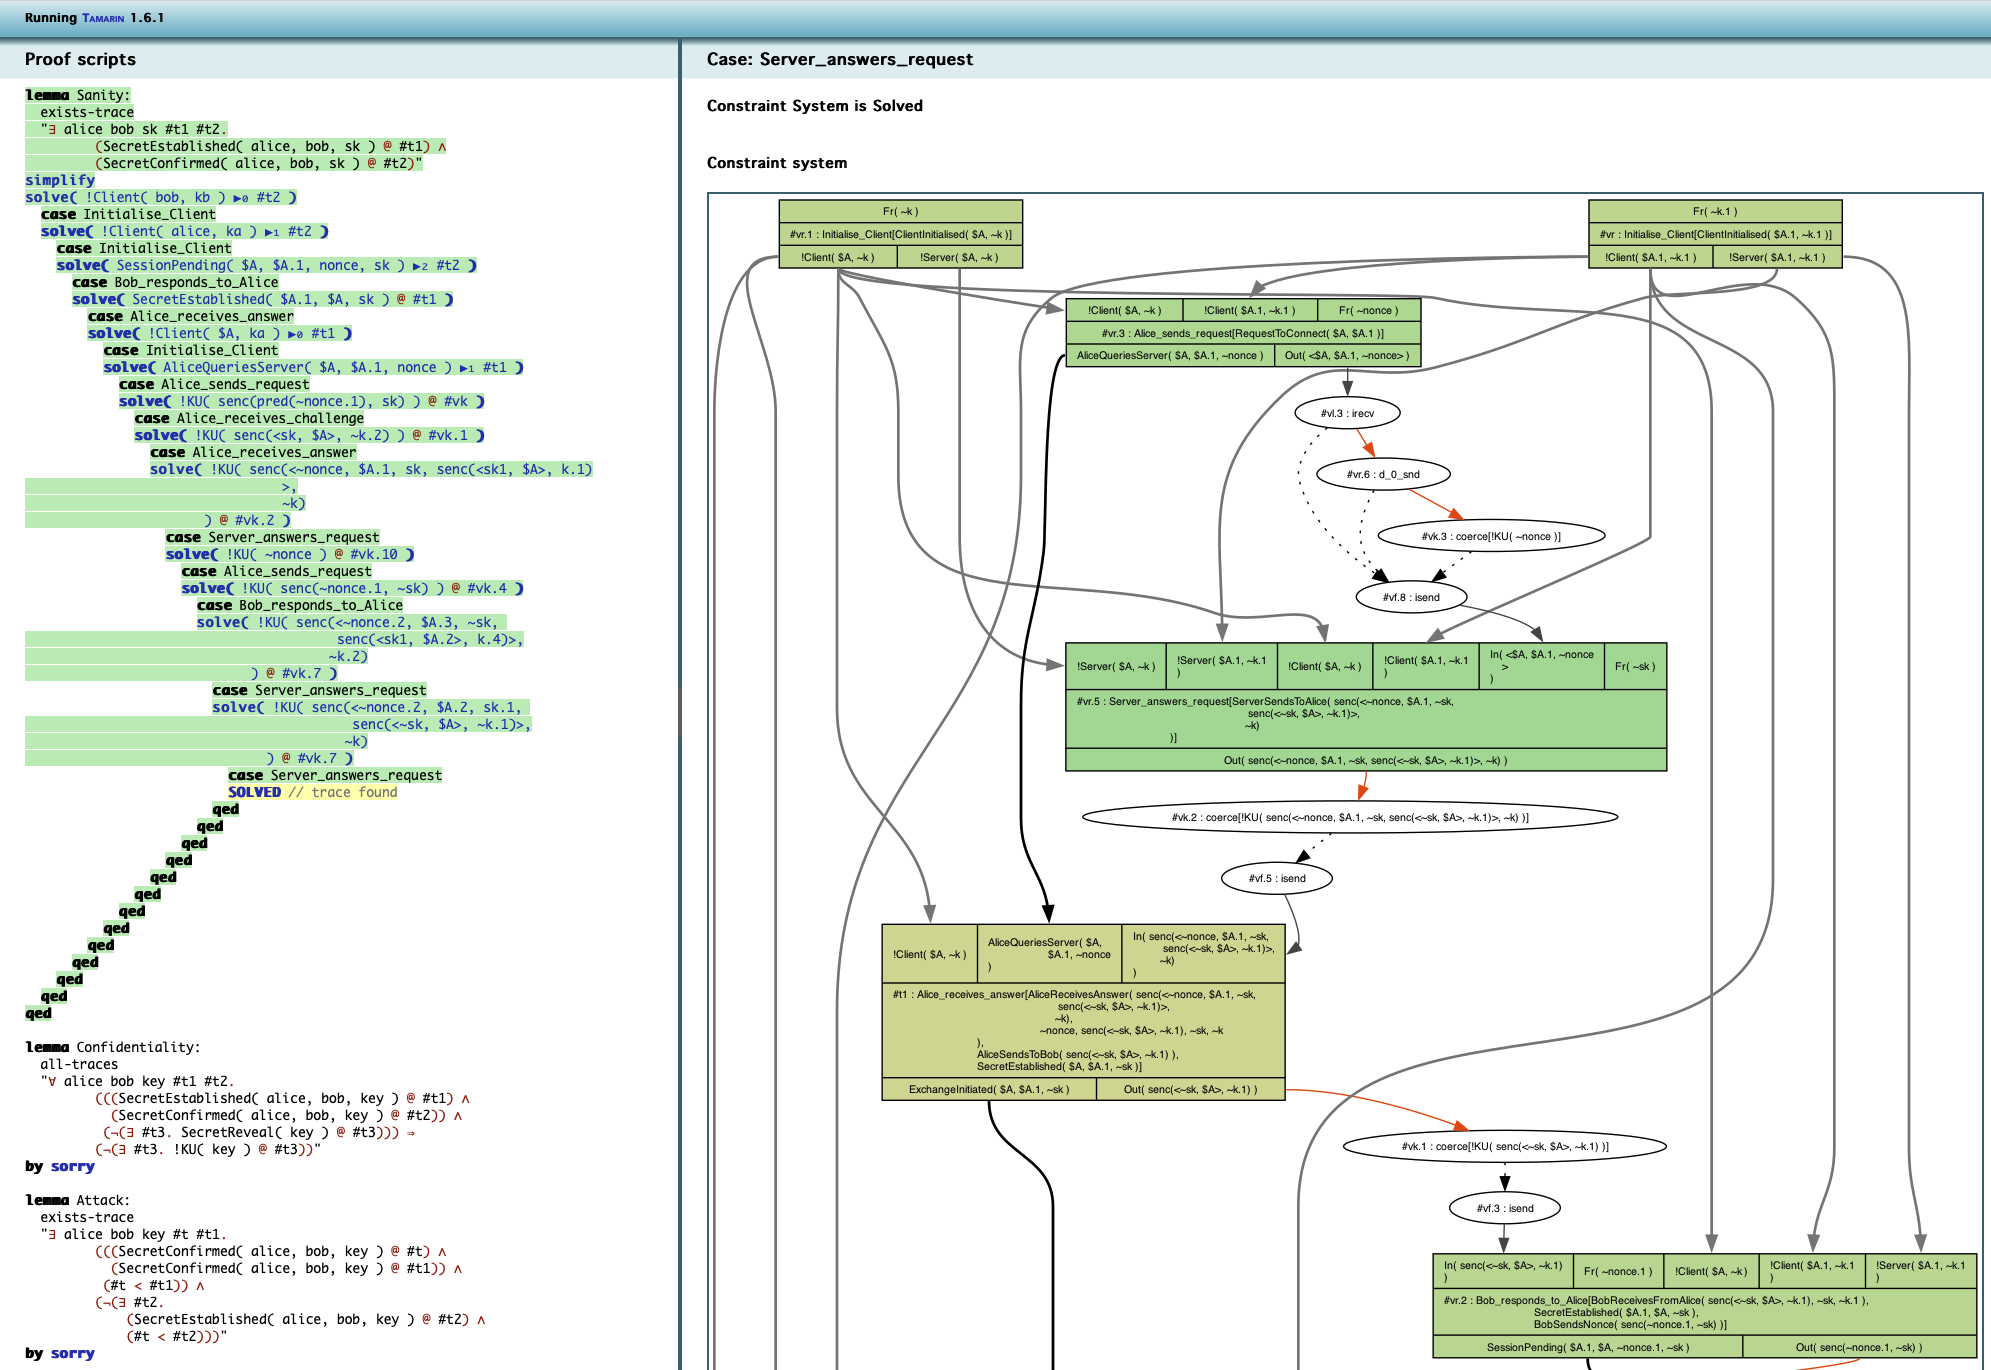
\includegraphics[width=0.8\textwidth]{images/gui.png}
    \caption{Tamarin's interactive mode}
    \label{fig:interactive}
\end{figure*}

\subsubsection{Restrictions}

Similarly to lemmas, \textit{restrictions} are specified through guarded fragments of first order logic. The difference between the two is that while lemmas express properties to prove, a restriction limits the possible traces of a protocol to the executions that satisfy the specified formula. An example of restriction use could be to avoid the application of the same rule twice:

\begin{gather*}
    [\mono{OldFact}(x)] \xrightarrow{\mono{OnlyOnce}()} [\mono{NewFact}(x)]\\
    \phi : \forall i,j : \mono{OnlyOnce}() @ i \land \mono{OnlyOnce} @ j \Rightarrow i = j
\end{gather*}

\subsubsection{Re-use lemmas}

Finally, the last functionality we introduce are \textit{re-use lemmas}: defined with the $\mono{[reuse]}$ keyword, these formulas, once proved, can be used by Tamarin in the demonstration of the subsequent specified lemmas.

%------------------------------------------------

\section{Formalizing Social Engineering attacks}\label{sec:SocialEngineering}

When verifying cryptographic protocols, we tend to abstract the parties involved in the exchanges to perfect machines which follow flawlessly the rules of the scheme under analysis. In practice, such operations are performed by humans, which are far for perfect and may introduce unexpected behaviours into the dynamics of a protocol (for example by falling for a social engineering attack), leading to possible catastrophical outcomes. In a recent report by Gitnux \cite{Gitnux_2023}, the authors state that

\begin{quote} Social engineering is a prevalent threat, with 90\% of data breaches having social engineering components and 62\% of businesses experiencing attacks \end{quote}

highlighting the fact that human error is a key element in real-world threat analysis that must be taken into serious consideration when examining security-oriented protocols. Several types of cyberattacks have been developed in recent times to exploit such vulnerability: a comprehensive summary of this field of research is available at \cite{Salahdine_2019}, from which we have taken Figure \ref{fig:social_engineering_attacks} for a quick reference.

\begin{figure}[htbp]
    \centering
    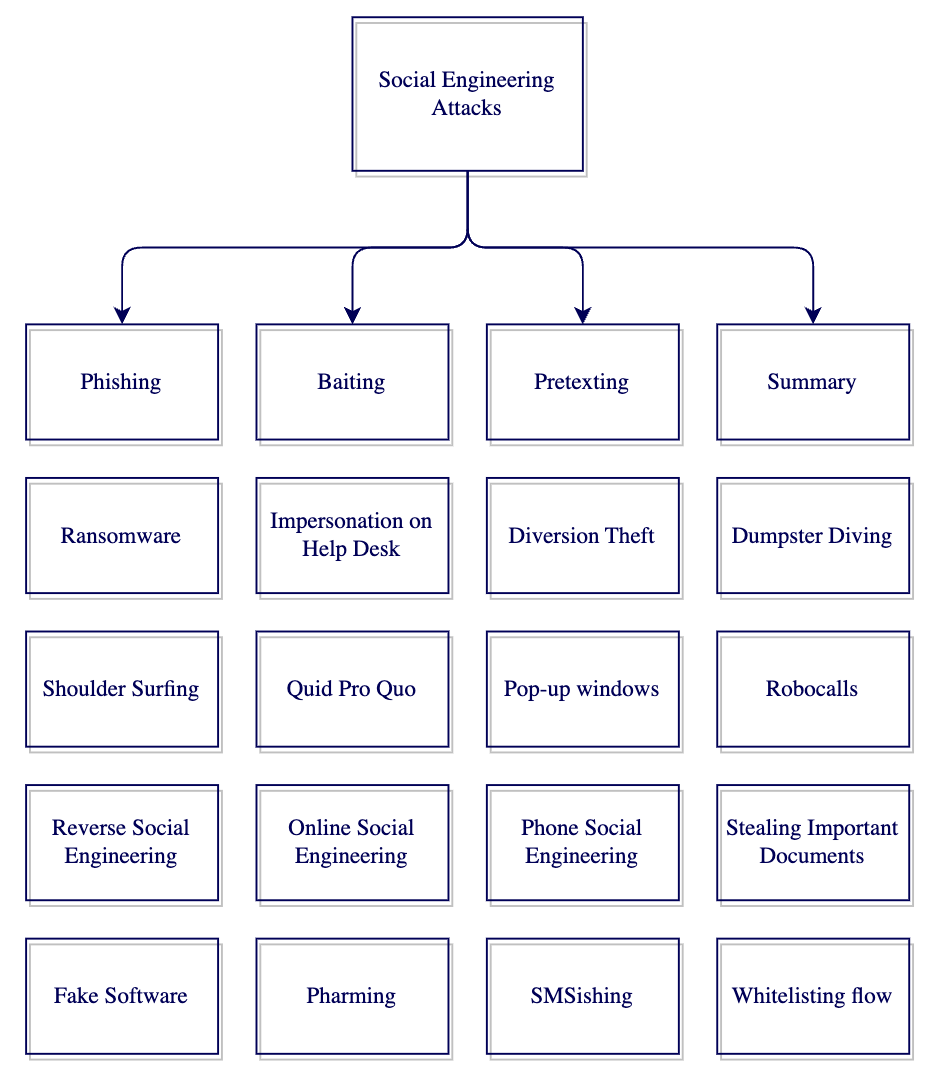
\includegraphics[width=0.5\textwidth]{images/socialengineeringattacks.png}
    \caption{Summary of the categories of Social Engineering Attacks. Image inspired by Figure 4 of \cite{Salahdine_2019}}
    \label{fig:social_engineering_attacks}
  \end{figure}
  
To narrow the gap between the attacks normally considered in formal protocol verification and the threat surface of actual implementation of said schemes, Basin et al. proposed in 2016 \cite{Basin_2016} an innovative solution to model erroneous deviations from protocol specification within the Dolev Yao model. In the rest of this section, we will introduce the ideas behind such article, underlining how simple it is to implement these ideas within Tamarin's fact rewriting mechanics. Note that the paper actually includes some results and notation from previous publications without prior introduction: to provide a more comprehensible explaination of the material we will include additional information also from articles \cite{Lowe_1997} and \cite{Basin_2015} and the appendixes of \cite{Basin_2016}, devoid of an explicit notice.

\subsection{Including human knowledge in protocol formalization}

Before defining errors in human behaviour, we need to actually establish which are the capabilities of said humans within our model. It is not unreasonable to presume that a person can perform simple operations but not complex computations unaided; in particular, we assume that a human can:

\begin{enumerate}
    \item Send and receive messages on specified channels
    \item Concatenate messages
    \item Split concatenated messages
\end{enumerate}

On the other hand, humans are not able to encrypt or decrypt messages unaided.

A key concept in this formalization is the concept of \textit{human knowledge}: each individual partaking to an exchange stores a set of (tagged) information initially defined at initialisation and then updated through the retrieval of new messages from the network. To generalise this idea, the authors suggest to unbound the number of information storable by any human partecipant and to model actual knowledge evolution through a database of facts in the form of $!HK(H, \langle t, x \rangle)$, where:

\begin{itemize}
    \item The fact is declared as persistent (through the juxtaposition of the exclamation mark) to portray that any information can be consumed infinitely many times
    \item $H$ is the human agent taken into consideration
    \item $t$ is the \textit{tag} for the data stored
    \item $x$ is the actual information known by $H$
\end{itemize}

The tag is required to denote the human's interpretation of messages: intuitively, we need to be able to distinguish between different types of information (passwords, emails, etc...), thus we have to define a recursive function that is able to associate a label to any term belonging to the term algebra $\mathcal{T}_{\Sigma}(X)$ we are taking into consideration. At first, we need to assume to have the additional injective function $t: \Sigma \cup X \to \mathcal{L}$ (where $\mathcal{L}$ is the alphabet of intermediate labels) which associates to any ground term and function symbol of our theory a unique, atomic tag. We can then use such function to define $T:\mathcal{T}_{\Sigma}(X) \to \mathcal{L^*}$ as:

\begin{align*}
    T(m) =
    \begin{cases}
        t(m) & \textrm{ if } m \in \Sigma \cup X \\
        t(f) \cdot T(a_1) \cdot ... \cdot T(a_n) & \textrm{ if } m = f(a_1, ..., a_n), f \textrm{ is a function symbol in } \Sigma \textrm{ and } a_i \in \mathcal{T}_{\Sigma}(X)
    \end{cases}
\end{align*}

where $\cdot$ is the concatenation operator. Our objective is to map the set of labels to the set of public constants $\mathcal{C}_\textrm{pub}$ included in the algebra itself. Since both $\mathcal{L^*}$ and $\mathcal{C}_\textrm{pub}$ are countably infinite sets, there must be an injective mapping from the first set to the latter. By composing such function with $T$, we obtain the function $preTag : \mathcal{T}_\Sigma(X) \to \mathcal{C}_\textrm{pub}$. The last step in our construction is to define the actual labelling map $tag : \mathcal{T}_\Sigma{X} \to \mathcal{T}_{\mathcal{C}_\textrm{pub} \cup \{\textrm{pair}\} }$ by including the possibility of term concatenation:

\begin{align*}
    Tag(m) =
    \begin{cases}
        \langle Tag(m_1), Tag(m_2) \rangle & \textrm{ if } m = \langle m_1, m_2 \rangle \\
        preTag(m) & \textrm{ otherwise }
    \end{cases}
\end{align*}

This additional step is done to allow humans to create new knowledge based on the concatenation of pre-existing information (remember that this operations is one of the few operations that individuals can perform unaided). The rules proposed by the authors require the use of such function work with the human-knowledge database facts $\mono{!HK}$: a generic information $x$ will be actually stored as $\mono{!HK}(H, \langle Tag(x), x \rangle)$.

Before continuing, it is helpful to define the $\vdash_H$ predicate, defined over pairs of tag-message pairs:
\begin{equation*}
    \langle t, m \rangle \vdash_H \langle t', m' \rangle \iff \exists i, k : 1 \leq i \leq k \land t = \langle t_1, ..., t_k \rangle \land m = \langle m_1, ..., m_k \rangle \land t' = t_i \land m' = m_i
\end{equation*}

Intuitively, $\langle t, m \rangle \vdash_H \langle t', m' \rangle$ if and only if agent $H$ can select $\langle t', m' \rangle$ from $\langle t, m \rangle$.

\subsection{Formalizing human errors}\label{sec:formalizing_human_errors}

From a global perspective, a cryptographic protocol is typically defined in some form of Alice and Bob notation. In particular, we are going to use an extended notation that differentiates the channels used for communication based the form of security they guarantee (in the following definitions, let us assume that we want to represent a channel between parties $A$ and $B$):

\begin{itemize}
    \item An \textit{insecure channel}: $A \ins B$
    \item An \textit{authentic channel}: $A \auth B$
    \item A \textit{confidential channel}: $A \conf B$
    \item A \textit{secure channel}: $A \sec B$
\end{itemize}

Do not forget that, although Tamarin only features insecure channels (the ones with the weakest assumptions) by default, but, as we showed in \ref{sec:DolevYaoRules} it is really easy to define rules to include also other types of channels.

If, on the other hand, we want to consider the actions perfomed by any agent specifically, we can focus on \textit{role scripts}. A role script for an agent $H$ in a given protocol is the sequence of operations that $H$ has to execute in order to successfully complete the run of the exchange on his side, thus we can see them as "projections" onto parties of entire protocol specifications. More formally, a role script is a sequence of \textit{events} $e \in \mathcal{T}_{\Sigma \cup \textrm{RoleActions}}(X)$, where $\textrm{RoleActions} = \{\mono{Send}, \mono{Receive}, \mono{Start}, \mono{Fresh} \}$, where the top-level function of $e$ belongs to $\textrm{RoleActions}$. Such functions have a well defined meaning:

\begin{itemize}
    \item $\mono{Send}(A,l,P,m)$ means that agent $A$ sends on a channel of type $l$ the message $m$ to the apparent party $P$
    \item $\mono{Receive}(A,l,P,m)$ means that agent $A$ receives from a channel of type $l$ a message with expected pattern $m$ from the apparent party $P$
    \item $\mono{Start}(A,t)$ indicates the initial knowledge of term $t$ by agent $A$
    \item $\mono{Fresh}(A,t)$ indicates that agent $A$ produces a fresh term $t$
\end{itemize}

A brilliant example of the projection of a protocol specification onto a role script is provided in the article:

\begin{figure}
\begin{alignat*}{3}
    &0.\  S &&: \textrm{knows}(R)\\
    &0.\  R &&: \textrm{knows}(S, m_2)\\
    &1.\  S \ins R &&: \textrm{fresh}(m_1).m_1\\
    &2.\  R \sec S &&: m_2
\end{alignat*}
\label{eq:toy_protocol}
\caption{Toy protocol in Alice and Bob notation}
\end{figure}

\begin{figure}
\begin{equation*}
    \langle \mono{Start}(S,R), \mono{Fresh}(S, m_1), \mono{Send}(S, \textrm{ins}, R, m_1), \mono{Receive}(S, \textrm{sec}, R, m_2) \rangle
\end{equation*}
\caption{Role script of role $S$ for the Toy protocol}
\end{figure}

In turn, any role script can be translated into a set of Tamarin rewriting rules that formalize the behaviour of the given party (in this case $S$) into the system:

\begin{gather*}
    [ \ ] \xrightarrow{\mono{Start}(S,R)} [\mono{AgSt}(S,0,R)]\\
    [\mono{AgSt}(S,0,R), \mono{Fr}(m_1)] \xrightarrow{\mono{Fresh}(S,m_1)} [\mono{AgSt}(S,1,\langle R,m_1 \rangle)]\\
    [\mono{AgSt}(S,1,\langle R,m_1 \rangle)] \xrightarrow{\mono{Send}(S,\textrm{ins},R,m_1)} [\mono{AgSt}(S,2,\langle R,m_1 \rangle), \mono{Out}_\textrm{ins}(\langle S, R, m_1 \rangle)]\\
    [\mono{AgSt}(S,2,\langle R,m_1 \rangle), \mono{In}_\textrm{sec}(\langle R, S, m_2 \rangle)] \xrightarrow{\mono{Receive}(S, \textrm{sec}, R, m_2)} [\mono{AgSt}(S,3,\langle R, m_1, m_2 \rangle)]
\end{gather*}

Assuming we have the corresponding rules also for $R$, we can see that a succesfull execution of the protocols that follows the specification of \ref{eq:toy_protocol} will induce a trace that mirrors the role script of an agent (given that we ignore the action facts belonging to other parties' actions). Furthermore, note that the function symbols belonging to $\textrm{RoleActions}$ are now used as action facts: this is natural since in Tamarin we can only specify formulas (within lemmas and restrictions) over facts and not directly over terms.

After formally introducing role scripts, we can define a human error as \textit{any deviation of a human from his role script}. Any human that makes mistakes is said a \textit{fallible human}. On the other hand, an agent which adheres perfectly to his specification is said an \textit{infallible human}.

Normally, in a formal verification context we would take into consideration only infallible humans. Such assumption would be reasonable for (almost) completely automatic protocols that necessitate little to no input by users and thus present slim chances of uncorrect executions. Conversely, when dealing with interactive protocols which require a lot of user intervention (for example any 2-factor authentication protocol) it is imperative to include the possibility that an agent makes a mistake, either because of carelessness or as a consequence of fraudolent attacker behaviour.

Fallible humans can be introduced through two main approaches (summarized in Figure \ref{fig:fallible_humans}), that we will now briefly explain.

\begin{figure}[htbp]
    \centering
    \includegraphics[width=0.9\textwidth]{images/falliblehumans.png}
    \caption{Approaches to introducing fallible humans. In the graphs, $I$ is the infallible human, $U$ is the untrained human and an edge from a node $N$ to a node $M$ denotes that $N$ induces a subset of the behaviours of $M$. Blue nodes are \textit{skilled humans} while teals nodes represent \textit{trained humans}. Image inspired by Figure 1 of \cite{Basin_2016}}
    \label{fig:fallible_humans}
\end{figure}

\subsubsection{Skilled Human Approach}

The \textit{Skilled Human Approach} starts by firstly taking into consideration an infallible human that does not drift from a given protocol's specification and then by introducing other humans, which can make a fixed number of mistakes (called \textit{skilled humans}). Each new agent introduced on the basis of another previous human induces a supersets of the latter's possible behaviours: in this approach, we weaken the infallible human until the security properties are not guaranteed anymmore. It is interesting to note that the data structure that naturally depicts this approach is not a sequence, but instead a directed acyclic graph: we can consider different routes while weakening our actors (for example, by allowing the agents to fall for a phishing mail or to skip a QR code verification, but not necessarily both of them together), thus we can find some (possibly different) minimal sets of actions that must be executed rigorously according to the protocol in order to avoid security concerns.

\subsubsection{Rule-Based Human Approach}

The \textit{Rule-Based Human Approach} begins with the introduction of an \textit{untrained human}, which is capable of executing any possible behaviour (for example, leaking passwords without concern, skipping any additional verification step, communicating verification codes received out-of-band to the attacker, etc ...) and then strengthens such agent by imposing restrictions on the acceptable actions. This formalization models a human that does not know the protocol specification but adheres to some basic guidelines (for example, it is sensible to assume that a user does not know the dynamics of an given protocol, but he is aware that he must not communicate passwords outside of the authenticated plaforms).

Within Tamarin's fact rewriting system it is quite natural to formalize humans through the rule-based approach: firstly, we can model the untrained human behaviour through the following rules:

\begin{gather}
    [\mono{Fr}(x)] \xrightarrow{\mono{Fresh}(H, \langle t,x \rangle)} [\mono{!HK}(H, \langle t,x \rangle)] \label{eq:fresh_term_knowledge}\\
    [\mono{!HK}(H, \langle t, x \rangle)] \xrightarrow{\mono{Send}(H, \textrm{ins}, P, \langle t,x \rangle)} [\mono{Out}_{\textrm{ins}}(\langle H, P, \langle t,x \rangle \rangle)] \label{eq:telling_the_attacker}\\
    [\mono{In}_{\textrm{ins}}(\langle P, H, \langle t,x \rangle \rangle)] \xrightarrow{\mono{Receive}(H, \textrm{ins}, P, \langle t,x \rangle)} [\mono{!HK}(H, \langle t,x \rangle)] \label{eq:retrieving_from_the_attacker}
\end{gather}

These rules clearly follow the semantics introduced in Section \ref{sec:formalizing_human_errors} when explaining Role Scripts. We can trivially define rules equivalent to \ref{eq:telling_the_attacker} and \ref{eq:retrieving_from_the_attacker} for the remaining types of channels ($\textrm{auth}, \textrm{conf}, \textrm{sec}$).

Let us take a closer look at these rules:

\begin{itemize}
    \item Rule \ref{eq:fresh_term_knowledge} allows to any human party to generate a fresh term and to add it to his knowledge, along with the relevant tag $t$. This models, for example, the generation of a new password by a registering user.
    \item Rule \ref{eq:telling_the_attacker} includes into the formalization the leakage of any information (both private and non) that makes up the human's knowledge database onto the network. A real-world example of this would be an involuntary password reveal by a user.
    \item Rule \ref{eq:retrieving_from_the_attacker} allows a human to update his existing knowledge based on new information received from the network. For example, an unexperienced user may receive a phishing mail explaining that he must re-enter his credentials into a new website because of security reasons.
\end{itemize}

Note that all of the rules have action facts equivalent to the function symbols belonging to $\textrm{RoleActions}$. This will allow us to introduce rules that constrain the possible behaviours (thus effectively defining skilled humans) by including additional restrictions in the theory\footnote{Note that here, technically, we are defining predicates. In practice, we implement them in Tamarin as restrictions, thus we will use these two terms interchangeably within the rest of this section}. Technically, it would be possible to include any constraint to limit the possible action executed by a human agent, but the authors propose 4 very generic formulas that cover many social engineering threats:

\paragraph{$\mono{NoTell}$ for avoiding leakage of private information}

If we wanted to prevent a user $H$ from revealing information labelled by $tag$ to the rest of the network (for example a private key in an asymmetric cryptography context) during the execution of protocol $P$ (intended as a set of protocol rewriting rules) we could include the following predicate (of course using the restriction construct):

\begin{equation*}
    \mono{NoTell}(H, tag) := \forall \mono{Send}(H, l, P, \langle t,m \rangle) \in tr \in traces(P), t', m' : \langle t, m \rangle \vdash_H \langle t', m' \rangle \Rightarrow t' \not = tag
\end{equation*}

This predicate ensures that $H$ will never send the information tagged with $t$ onto the network. Of course, this restriction can not be imposed on \textit{all} private information of agent $H$: during authentication procedures, for example, a user may be legitimaetly prompted for the input of a password and this constraint would not allow it. For this reason, the following restriction has been introduced.

\paragraph{$\mono{NoTellExcept}$ for safe communication of credentials}

Let us assume that we have an action fact $\mono{InitK}(H, \langle tag, x \rangle)$ that generalizes the $\mono{Start}$ action by denoting the knowledge of agent $H$ of the term $x$ with tag $t$ at initialisation. We can exploit such fact to limit the human to only reveal \textit{some} secret information to trusted parties over secure or authenticated channels:

\begin{align*}
    \mono{NoTellExcept}(H,&tag,rtag) := \forall \mono{Send}(H,l,P,\langle t,m \rangle) \in tr \in traces(P), m', R : \\
    &\mono{InitK}(H, \langle rtag, R \rangle) \in tr \land \langle t,m \rangle \vdash_H \langle tag, m' \rangle \Rightarrow P = R \land (l=\textrm{sec} \lor l = \textrm{conf})
\end{align*}

This predicate ensures that all information labelled by $tag$ is shared only with parties that we trust (since we include them in our initialisation knowledge). A practical implementation of this within a theory could require, for example, that any message labelled by the tag $\textrm{'password'}$ is only shared with an authentic platform (of which we know the URL saved under the tag $rtag$).

\paragraph{$\mono{NoGet}$ for protecting information integrity}

A user may be tricked by an attacker to update pre-existing (safety) information (for example through a realistic spear-phishing attack). It is not unrealistic, though, to assume that a reasonably cautious user may refrain to believe some new data regarding sensitive information received from the network. This situation can be modelled through the following predicate:

\begin{equation*}
    \mono{NoGet}(H,tag) := \forall \mono{Receive}(H,l,P,\langle t,m \rangle) \in tr \in traces(P), t', m' : \langle t, m \rangle \vdash_H \langle t', m' \rangle \Rightarrow t' \not = tag
\end{equation*}

Such constraint prevents any piace of knowledge tagged by $tag$ to be updated from information retrieved from the network. A practical example of this would be to assume that an antivirus' customers only use the software built-in update mechanics and avoid accepting new "update links" received from internet.

\paragraph{$\mono{ICompare}$ to enforce important security checks}

Some protocols like MTProto2 are relatively safe under the assumption of users checking QR codes for encryption to ensure the absence of Man-In-The-Middle attacks \cite{Miculan_2023}. If we wanted to enforce similar checks within our system, we could include the following predicates:

\begin{align*}
    \mono{ICompare}(H,tag) := \forall \mono{Rec}&\mono{eive}(H,l,P,\langle t,m \rangle) \in tr \in traces(P), m' : \\
    &\langle t,m \rangle \vdash_H \langle tag,m' \rangle \Rightarrow \mono{InitK}(H, \langle tag,m' \rangle) \in tr
\end{align*}

Intuitively, this predicate requires that any piece of information received from the network and labelled with $tag$ must be checked against the agent's initial knowledge.

\paragraph{Other predicates}

While the predicates proposed by the article cover a lot of real world scenarios, the list is far from comprehensive: for example, one may want to generalize the $\mono{NoTellExcept}$ restriction in order to allow an authenticated party to communicate to the user another trust platform with which he can share private information, or it may be useful to have define the $\mono{NoGet}$ predicate in order to avoid updating also knowledge created during the exchange and not only at initialisation. In any case, it is clear that extending a theory with such constraints is far from complex.

\paragraph{Proving properties}

The most convenient aspect of this approach is the fact that, by including the constraints on the behaviour of the untrained human through predicates, we can easily keep our usual formulas for the properties to check while quickly sweeping in or out the restrictions in order to verify different scenarios. Furthermore, by including the reference to the a particular human $H$ within our predicates we are able to impose different degrees of freedom to various agents for a more general (and capillary) verification strategy. In particular, our approach distinguishes a particular human $H$ for whom security properties are analyzed, while allowing an arbitrary number of untrained (or less skilled) humans in the network to verify whether errors of external parties may affect $H$'s security guarantees.

\section{Conclusions}\label{sec:Conclusions}

In this article we firstly introduced the general problem of automated verification of cryptographic protocols in the Dolev Yao model, then we gave a general overview of the Tamarin Prover, mainly from a user's perspective. Although such outline covered most of the features provided by the tool, for a more comprehensive look at the subject we suggest consulting \cite{tamarinManual}. Finally, we showed how to include various Social Engineering attacks within the considered threat model by formalizing human knowledge and agent errors through multisets rewriting rules and restrictions. This allows us to verify protocols that rely on multiple interactions with the users in a more realistic and complete way. Possible future works would include the development of additional predicates to model further assumptions and the ideation of a concrete system to implement the skilled humans approach.

\bibliographystyle{alpha}
\bibliography{references}

\end{document}